%!TEX root = main.tex

Figure \ref{fig:domain_model} outlines the most significant entities taking part in or being used by the Easy Ticketing system. The system components and their interactions are presented alongside the main external entities needed for different functionalities of the system. The figure also introduces the main actors responsible for the use cases presented in chapter \ref{chp:usecases}.

\begin{figure}[H]
	\centering
	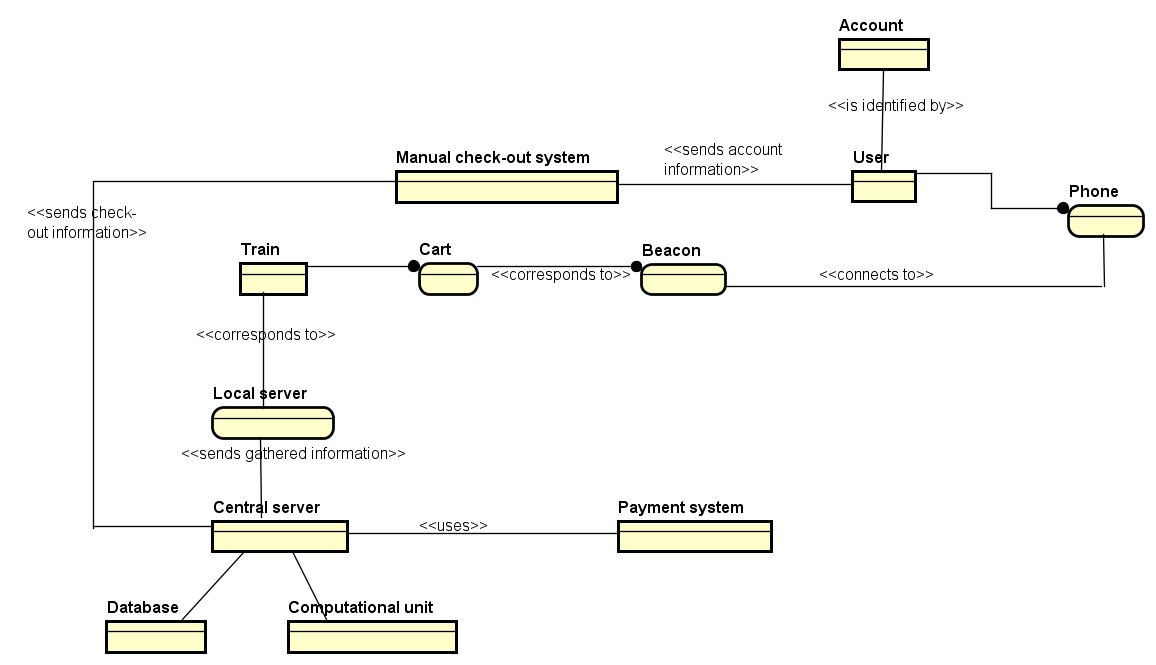
\includegraphics[width=\textwidth]{Pictures/domain_model.png}
	\caption{Domain model}
	\label{fig:domain_model}
\end{figure}

The Easy Ticketing system can be divided into three main sets of components:
\begin{itemize}
	\item Main central server component
	\item Data retrieval component
	\item Mobile application
\end{itemize}

The main central server component will be responsible for two main tasks, namely data storage and data analysis. The data storage component will be represented by a centralised database containing information related to all user accounts, payments, trips, etc. The data analysis component will use an external payment system in order to perform financial transactions related to each trip. The computation of the price for each journey will be performed using several computational algorithms. The data analysis component will also receive and manage requests directly from the users related to displaying payments or trip related information specific for that user.

The data retrieval component will be represented by the components located inside the trains. These components will be divided into two sets: beacons and local servers. The beacons will initiate connections with all users located inside the train at a certain moment and retrieve information related to their accounts. Once all users have been identified, they will send this information to the local server component. This component will be responsible for transferring the collected information towards the main server component, once for each stop. If a connection to this component is not available, the local server will store the information locally until the connection is established.

The mobile application will be installed on the user's Smartphone and will enable the connection between the phone and the beacons. It will also store information related to the user's account(related to user identification) and information regarding the identification of beacons currently part of the system(this will enable the mobile application to check the validity of the beacon before sending sensitive information regarding the user's account).

The manual check-out system displayed in figure \ref{fig:domain_model} will be used as a back-up solution for checking out of a journey when the connection between the beacons and the mobile application is no longer available(e.g due to battery issues). Once the user leaves the train, he/she will be able to use this system located in the train station by logging in with their credentials and manually checking out of the trip.